\documentclass[12pt, TexShade, letterpaper]{report}

\usepackage{import}
\import{}{preamble.tex}

\begin{document}

\begin{titlepage}
		\begin{center}
			\vspace*{0.5cm}

			\LARGE
			\textbf{Analysis of 2x2 Cross-Over Trials}
			
			\vspace{1cm}
			
			\textit{Jules Lanari-Collard}
			
			\vspace{1.2cm}
			
			
\includegraphics[width=0.25\textwidth]{mcglogo.png}
			
			\Large
			MATH 410 Final Report
			
			\vspace{-5mm}
			McGill University
			
			\vspace{-5mm}
			Montr\'eal, Qu\'ebec, Canada
			
			\vspace{5mm}
			August 16, 2024
			\small
			\vspace{0.5cm}
			{\color{red} \hrule height 0.75mm}
			
			\vspace{0.2cm}
			
			Supervised by Dr. José Correa
		\end{center}
\end{titlepage}

\setlength{\voffset}{2cm}
\renewcommand{\chaptermark}[1]{%
	\markboth{\thechapter.\ #1}{}}
\chapter*{Abstract}\markboth{Abstract}{}
	\label{chap:engAbstract}
%	\addcontentsline{toc}{section}{\nameref{chap:engAbstract}}

 % Start of ToC, LoT, gls
	\tableofcontents\thispagestyle{plain}

 	\clearpage
	\pagenumbering{arabic} % restart page numbers at one, now in arabic style

	% start of mainmatter
\chapter{Introduction to Cross-over Trials}
\section{The Cross-over Design}
A cross-over trial is defined as a "trial in which subjects are given sequences of treatments with the object of studying differences between individual treatments" \cite{senn2002crossover}. This differs from the traditional parallel group trial, where subjects typically only receive one treatment throughout the trial.

The most common and simple cross-over design, is the 2x2 cross-over design, whereby there exist two treatments and two treatment groups. In this design, for example comparing two treatments \textit{A} and \textit{B}, subjects receive either \textit{A} or \textit{B} in the first period, and then are 'crossed over' to the other treatment in the second period. When only investigating the effects of one treatment (as opposed to comparing two treatments), the other 'treatment' is then a placebo.

Cross-over designs are typically used for testing treatments for ongoing or chronic diseases, where "there is no question of curing the underlying problem which has caused the illness but a hope of moderating its effects through treatment" \cite{senn2002crossover}. Examples of such conditions include asthma, rheumatism, epilepsy and migraines. Due to time constraints and the risk of drop-out or carryover, cross-over designs are more suitable to single-dose trials, as opposed to trials involving multiple doses over a period of time \cite{senn2002crossover}.

\subsection{Consequences}
A unique characteristic of the cross-over design is that only the \textit{order} of treatment is randomised, which has the following consequences \cite{piantadosi2005clinical}:
\begin{itemize}
    \item The validity of treatment comparison does not depend on randomisation.
    \item Randomisation does not guarantee an unbiased comparison of treatments.
    \item Treatment groups differ with respect to their recent exposure to potentially effective treatments.
\end{itemize}
In conclusion, the primary issue is that the comparability of treatments is not guaranteed by the structure of the trial alone, but instead depends on the treatments themselves \cite{piantadosi2005clinical}.

\section{Advantages}
The principal advantage of a cross-over design is that it can lead to significant savings in resources \cite{senn2002crossover}. Firstly, when compared to a parallel group trial, a cross-over design only requires half as many subjects to obtain the same number of observations per treatment.

Secondly, the data can be interpreted in terms of subject-level \textit{difference to control}, eliminating between-patient variation \cite{senn2002crossover}, which is usually greater than within-patient variation \cite{piantadosi2005clinical}. This reduces the number of observations (and hence subjects) required for the same precision in estimation. Furthermore, within-subject responses to treatments are usually positively correlated \cite{piantadosi2005clinical}, reducing the variance of the estimated treatment difference (from control) and increasing efficiency, as demonstrated below:

\begin{quote}
    \textit{Noticing that:}
\end{quote}
\begin{equation*}
    cov(\bar{Y}_A, \bar{Y}_B)
= \rho_{AB}sd(\bar{Y}_A)sd(\bar{Y}_B) = \rho_{AB} \cdot \frac{\sigma}{\sqrt{n}} \cdot \frac{\sigma}{\sqrt{n}} = \rho_{AB}\frac{\sigma^2}{n}
\end{equation*}
\begin{quote}
    \textit{Assuming constant variance in observations between patients and no period or carryover effects, we then have:}
\end{quote}
\begin{align*}
    var(\hat{\delta}_{AB}) &=
    \frac{\sigma^2}{n} + \frac{\sigma^2}{n} - 2cov(\bar{Y}_A, \bar{Y}_B) \\
    &= 2\frac{\sigma^2}{n}(1-\rho_{AB})
\end{align*}
\begin{quote}
    \textit{Where $\sigma^2$ is the observation variance, $\bar{Y}_A$ and $\bar{Y}_B$ are the average observations for treatments A and B respectively, $\rho_{AB}$ is the within-subject response correlation, and $\hat{\delta}_{AB} := \bar{Y}_A - \bar{Y}_B$.}

    Given that $\rho_{AB} = 0$ in parallel group trials, positive correlation of within-subject responses will make a crossover trial more efficient \cite{piantadosi2005clinical}.
\end{quote}

An oft-overlooked benefit to the crossover trial is improved recruitment and reduced spill-over rates \cite{piantadosi2005clinical}. Since all subjects are guaranteed to receive each treatment at least once, it can be easier to recruit participants. Furthermore, if a treatment is known to be desirable (e.g. exercise), parallel group trials can be subject to spill-over, where subjects in the control group voluntarily take the treatment. Cross-over trials are evidently less at risk of this, since all subjects know they will receive the treatment.

\section{Disadvantages}
Many of the aforementioned benefits of the crossover design come with drawbacks. For example, the longer trial and multiple treatments could be seen as an added inconvenience to patients, and analysis of results is often more difficult and complex (particularly when there are more than two treatments or groups). Also, the design cannot be used for infectious diseases, where either a significant deterioration or improvement in condition can occur during treatment, introducing bias into the subsequent treatment period. Patient drop-out is also very harmful to cross-over trials, since observations for all treatments are required for each patient to analyse the within-patient differences. In comparison, a parallel group trial can still recover some information after a patient drops out \cite{senn2002crossover}.

There is also risk of \textit{period-by-treatment interaction} complicating analysis, where the effect of the treatment is not constant over time \cite{senn2002crossover}. In other words, when the period in which the treatment is administered affects the effectiveness of the treatment.

\subsection{Carryover}
The most common example of a period-by-treatment interaction is carryover, defined as "the persistence of a treatment applied in one period in a subsequent period of treatment" \cite{senn2002crossover}. In a cross-over design, this occurs when at the beginning of the second treatment period, patients are not in the state they would have been in, had they not received treatment in the first period. This causes the effect of one treatment to be misinterpreted as the effect of both treatments combined, introducing bias to the treatment effect estimates.

Carryover is both difficult to test for and then to adjust for. Tests for carryover effects are difficult to interpret independently of the treatment effect, and including carryover parameters in the model introduces additional uncertainty and requires additional (usually unreasonable) assumptions \cite{senn2002crossover}.

\subsection{Wash-out Period}
Senn [2002] proposes that the most efficient way to deal with carryover is introducing a \textit{wash-out period} to the experiment design. A wash-out period is "a period in a trial during which the effect of a treatment given previously is believed to disappear" \cite{senn2002crossover}. After the wash-out period, we can assume that all measurements taken are no longer affected by the previous treatment, the consequence being that all conclusions become conditional on the absence of a carryover effect.

\chapter{Summary \& Visualisation of Cross-over Data}
This chapter will follow example data from Jones and Kenward \cite{jones2003design}, on a study testing efficacy of a drug (A) and a placebo (B) on patients with \textit{chronic obstructive pulmonary disease} (COPD). Due to the nature of the condition, the observation measurement used was \textit{peak expiratory flow rate} (PEFR), defined as "a simple measure of the maximal flow rate that can be achieved during forceful expiration following full inspiration" \cite{peakflowrate2023}. The study employed a 2x2 cross-over design on 56 patients, where each patient measured their PEFR 3 times per day during the treatment periods, recording the highest value. A sub-sample of the data is outlined in table \ref{pefData}.

\begin{table}[h]
\centering
\caption{Mean PEFR (L/min)}
\centering
\begin{tabular}[t]{l|l|l|r|r}
\hline
\textbf{Sequence} & \textbf{Subject} &
\textbf{Subject Label} & \textbf{Period 1} & \textbf{Period 2}\\
\hline
AB & 1 & 7 & 121.905 & 116.667\\
\hline
AB & 2 & 8 & 218.500 & 200.500\\
\hline
AB & 3 & 9 & 235.000 & 217.143\\
\hline
AB & 4 & 13 & 250.000 & 196.429\\
\hline
AB & 5 & 14 & 186.190 & 185.500\\
\hline
AB & 6 & 15 & 231.563 & 221.842\\
\hline
AB & 7 & 17 & 443.250 & 420.500\\
\hline
AB & 8 & 21 & 198.421 & 207.692\\
\hline
AB & 9 & 22 & 270.500 & 213.158\\
\hline
AB & 10 & 28 & 360.476 & 384.000\\
\hline
\end{tabular}
\label{pefData}
\end{table}
\section{Summarising Results}
When the outcome data is continuous, a simple summary table showing the mean and standard deviation of the outcomes \cite{vetter2017descriptive}, grouped by sequence and period (see table \ref{summaryTable}), suffices to give an overview of the data.  If further data were collected on additional covariates, they can be summarised using the traditional \textit{Table 1}.
\begin{table}
\centering
\caption{PEFR Results Summary (L/min)}
\centering
\begin{tabular}[t]{l|r|r|r|r|r}
\hline
Sequence & Subjects & Mean PEFR Period 1 & SD PEFR Period 1 & Mean PEFR Period 2 & SD PEFR Period 2\\
\hline
AB & 27 & 245.8387 & 82.77956 & 239.2033 & 81.69683\\
\hline
BA & 29 & 215.9919 & 72.62905 & 230.1617 & 73.94153\\
\hline
\end{tabular}
\end{table}


\section{Summary Plots}
Before undertaking any analysis, it is important to gain an understanding of the data and preliminary results. This section demonstrates the introductory plots suggested by Jones and Kenward \cite{jones2003design} for cross-over trials.

The first plot is a simple scatter plot of observations in each period, separated by group, as demonstrated in figure \ref{fig:period2vsperiod1}. Also included is a straight line with slope 1 and intercept 0; if the treatments were identical we would expect all observations to lie along this line. Using this plot we can verify within-patient correlation, and also notice the spread of points across the line, indicating between-patient variation.

\begin{figure}[h]
    \centering
    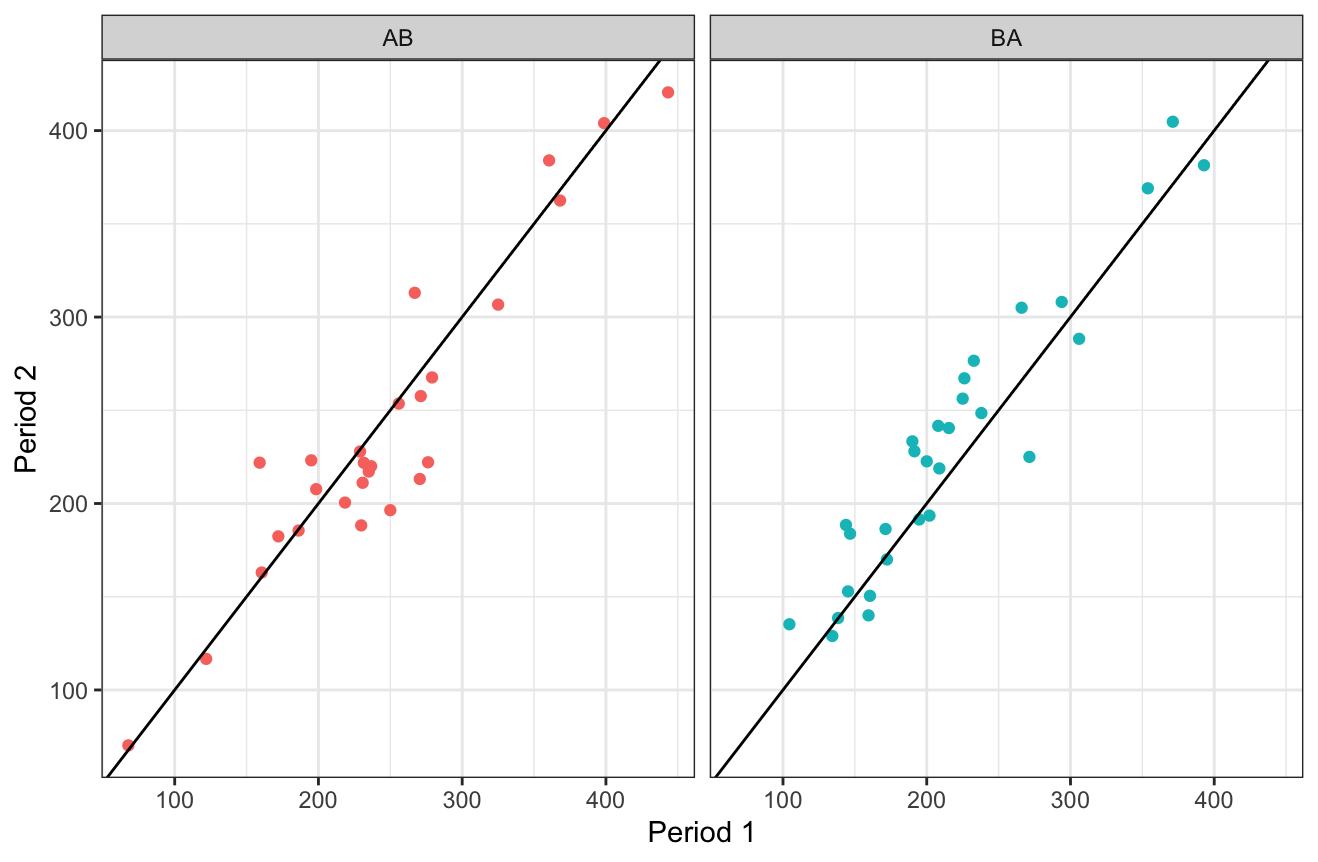
\includegraphics[width=0.85\linewidth]{report/figures/periodsPlot.png}
    \caption{Period 2 vs Period 1 Plots}
    \label{fig:period2vsperiod1}
\end{figure}

Additionally, we can overlay these plots, distinguishing the groups using colour (or shape), and also including the centroids for each group, as demonstrated in figure \ref{fig:centroids}. This allows us to make some preliminary conclusions:
\begin{itemize}
    \item Both groups appearing symmetrical about the diagonal line suggests absence of a period effect.
    \item Centroids appearing on opposite sides of the line, with some vertical separation, suggests there exists a direct treatment effect.
\end{itemize}

\begin{figure}[h]
    \centering
    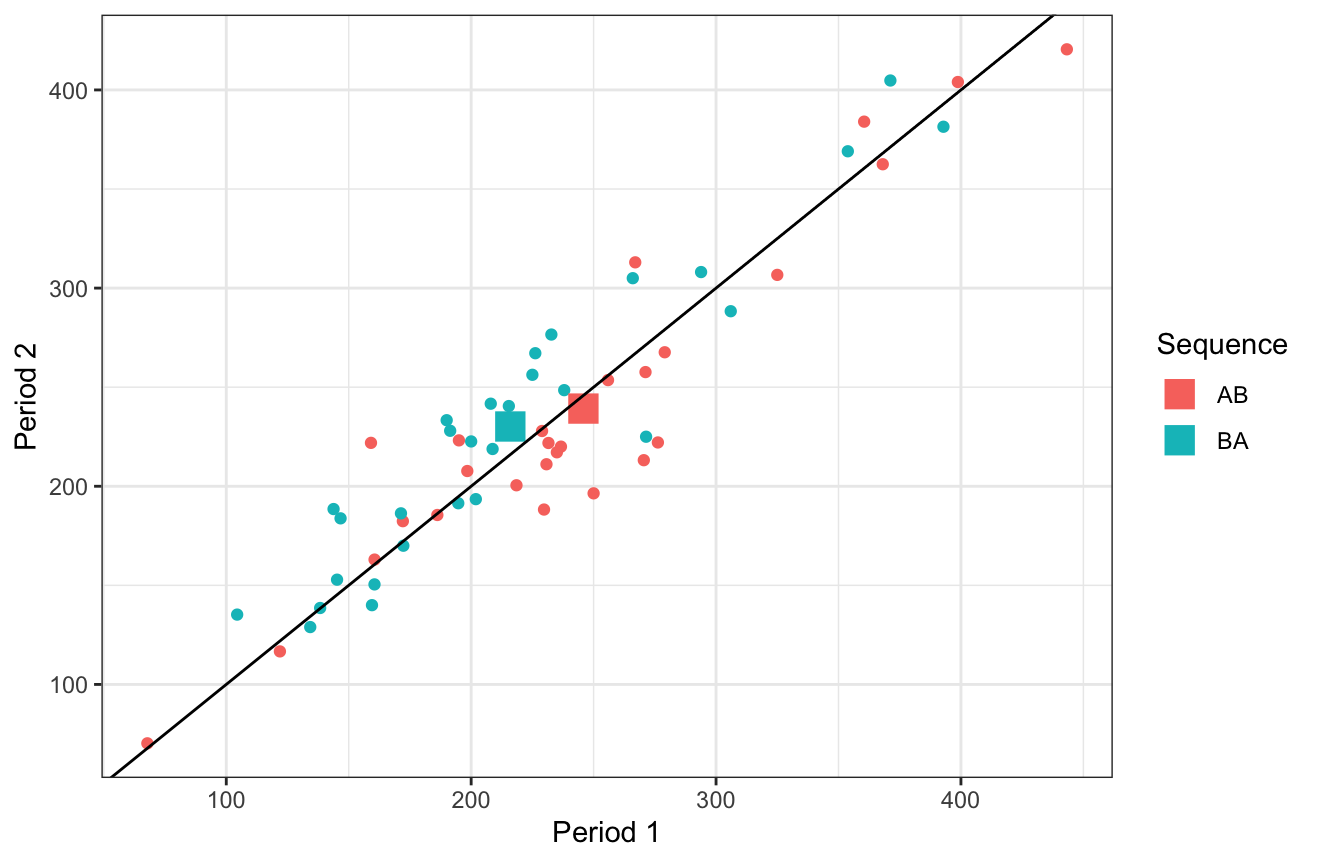
\includegraphics[width=0.85\linewidth]{report/figures/centroidsPlot.png}
    \caption{Period 2 vs Period 1 with Centroids}
    \label{fig:centroids}
\end{figure}

A plot which clearly shows the within-patient differences is the subject-profile plot, demonstrated in figure \ref{fig:subjectprofile}. This plot also allows us to visualise both within-patient and between-patient variability.

\begin{figure}[h]
    \centering
    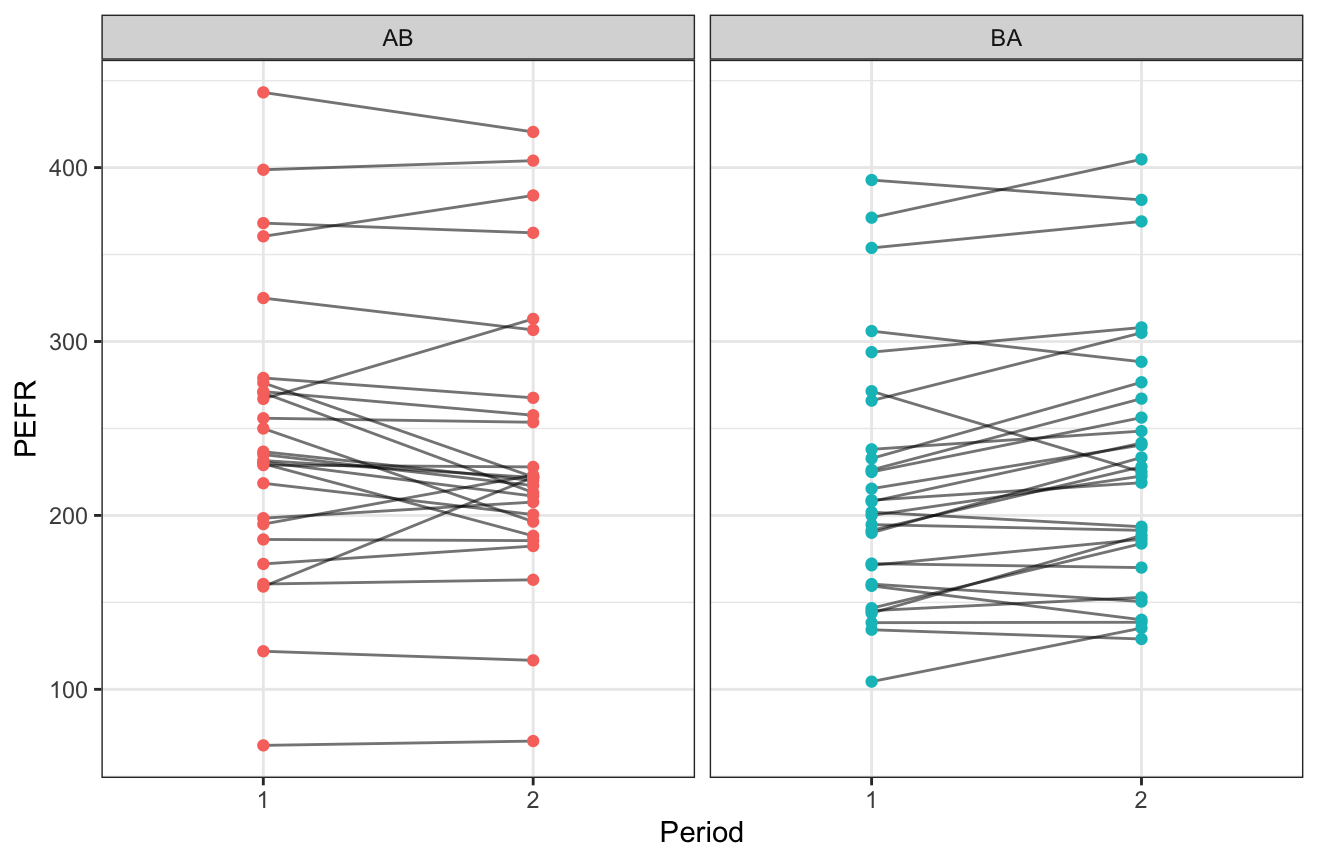
\includegraphics[width=0.85\linewidth]{report/figures/subjectProfilesPlot.png}
    \caption{Subject-Profile Plot}
    \label{fig:subjectprofile}
\end{figure}

Finally, the summary table \ref{summaryTable} can be visualised using a groups-by-periods plot, as shown in figure \ref{fig:groupsbyperiods}.
\begin{figure}[h]
    \centering
    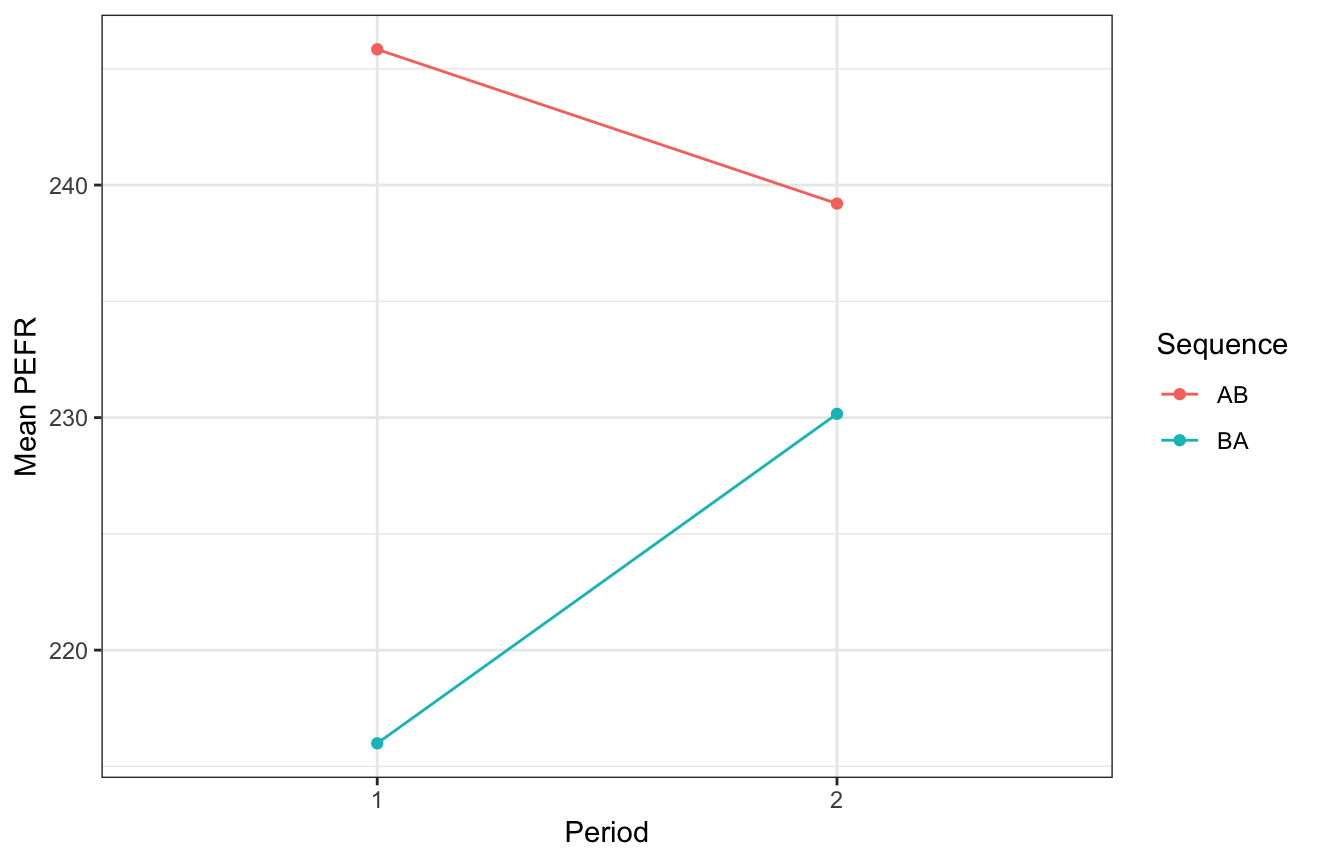
\includegraphics[width=0.85\linewidth]{report/figures/groupsByPeriodsPlot.png}
    \caption{Groups-by-Periods Plot}
    \label{fig:groupsbyperiods}
\end{figure}

\chapter{Analysis for Cross-over Trials}

\section{Matched-Pairs \textit{t}-Test}
The most straightforward analysis for a 2x2 cross-over trial uses a matched-pairs \textit{t}-test, which takes advantage of the paired structure of the data (every observation in period 1 can be matched to the subject's corresponding observation in period 2) \cite{senn2002crossover}. First we will introduce some basic notation:
\begin{itemize}
    \item $n$: number of subjects
    \item $y_{A_k}$, $y_{B_k}$: measured outcomes for subject $k$ ($k=1,\cdots,n$) after treatments $A$ and $B$ respectively.
    \item $d_k$: cross-over difference (i.e. difference between treatments), defined as $d_k := y_{A_k}-y_{B_k}$.
\end{itemize}
And then the mean cross-over difference $\bar{d} := \frac{1}{n}\sum_{i=1}^{n}d_k$ is an estimator for the true treatment effect (or difference) $\tau$. The matched-pairs \textit{t}-test then simply involves testing the hypothesis $H_0: \tau = 0$ against $H_1: \tau \neq 0$, by computing a t-statistic and comparing it against the corresponding critical value \cite{senn2002crossover}:
\begin{align*}
    \bar{d} &:= \frac{1}{n}\sum_{i=1}^{n}d_k \\
    s &= \sqrt{\frac{1}{n-1}\sum_{i=1}^{n}(d_k-\bar{d})^2} \\
    \widehat{se(\bar{d})} &= \frac{s}{\sqrt{n}} \\
    \implies \frac{\bar{d}}{\widehat{se(\bar{d})}} &\sim t_{n-1}
\end{align*}

\subsection{Assumptions}
This method involves two important assumptions:
\begin{itemize}
    \item Cross-over differences $d_k$ are independently and randomly distributed about the true treatment effect $\tau$.
    \item Cross-over differences $d_k$ are distributed approximately normally.
\end{itemize}
The most important assumption is the first one, and there are a number of situations which could cause the assumption to be violated:
\begin{itemize}
    \item Period effect
    \begin{itemize}
        \item There is a trend over time affecting the experiment \textit{as a whole}.
    \end{itemize}
    \item Period-by-treatment interaction
    \begin{itemize}
        \item Effect of treatment varies with the period in which it is given.
    \end{itemize}
    \item Carryover
    \item Patient-by-treatment interaction
    \begin{itemize}
        \item Effect of treatment varies by patient.
    \end{itemize}
    \item Patient-by-period interaction
    \begin{itemize}
        \item Patients are subject to period effects, which vary from patient to patient.
    \end{itemize}
\end{itemize}
Presence of a period effect artificially inflates the variance of cross-over differences, and under unbalanced allocation between treatment groups it introduces bias in the treatment effect estimates.

\section{Linear Mixed Model}

\section{Adjusting for Baseline Values}

	% Begin Bibliography
	{
	
	\bibliography{references}
	\bibliographystyle{ieeetr}
	
	}
	
\end{document}
